% TODO add tech / software table?
\section{Materials and methods}
In this section I will describe the development of the interactive visualization
as well as the process of gathering information on how people use it.

\subsection{Study design}

The study constitutes two main parts:
the development of the map presentation and
the survey on how people use the presentation.
The purpose of the development process is, of course, to produce the map presentation,
but just as importantly to enable the survey on how the interactive map is used.
This means that the development process and the survey are very dependent on each other,
and, should be approached as such.

This is why the first decision I made in regard to
the development of the interactive map
was to approach all its components as a whole.  % TODO talk briefly agile here or background?
The first step of the study is
to produce a minimal working state of the entire system,
where all of its components are integrated and work together.
My goal with this approach is twofold:
\begin{enumerate}
	\item Gain an understanding of the available tools and see whether the system, and by extension, the study, is realistic.
	\item Pinpoint major issues and the performance bottlenecks of the system as early as possible.
\end{enumerate}

Acquiring this knowledge as early as possible is essential.
It makes it possible for me to avoid wasted effort and, most importantly,
make sure I am developing a system that is valuable to the study.

After producing the minimal implementation I utilize an iterative approach
in developing the map presentation.
This means that I gradually improve the system on all of its aspects,
while constantly maintaining a functional state of the system.
Perhaps the largest value this approach brings is that it allows for
gradual improvement on the entire study.
Firstly, seeing the system take shape as functional whole
instead of separate components allows me to
continuously improve the relevancy of my research.
I say this not only in the context of gaining valuable results to my research questions --
I want to emphasize that to even know what research questions to ask is impossible with a linear approach.
Secondly, this kind of approach allows me to consider
the map and its functionalities from the perspective of the map user as early as possible,
better integrating the designing process of the survey into the study.
This is important as the map presentation is simultaneously an output of the development process
and an input to the design of the survey.

While the development process and the survey are linked to each other,
they each have their separate goals and outputs.
In addition to producing the map presentation,
the development process has the primary goal of providing the framework
that allows me to test and answer my research questions
about the making of an interactive map.
The goal of the survey is to gain insight on
how the interactive map works as a representation of the mapped phenomenon.
With the survey I collect data on map usage,
which I in turn analyse to answer my research questions related to the map usage.

\begin{figure}[H]
	\centering
	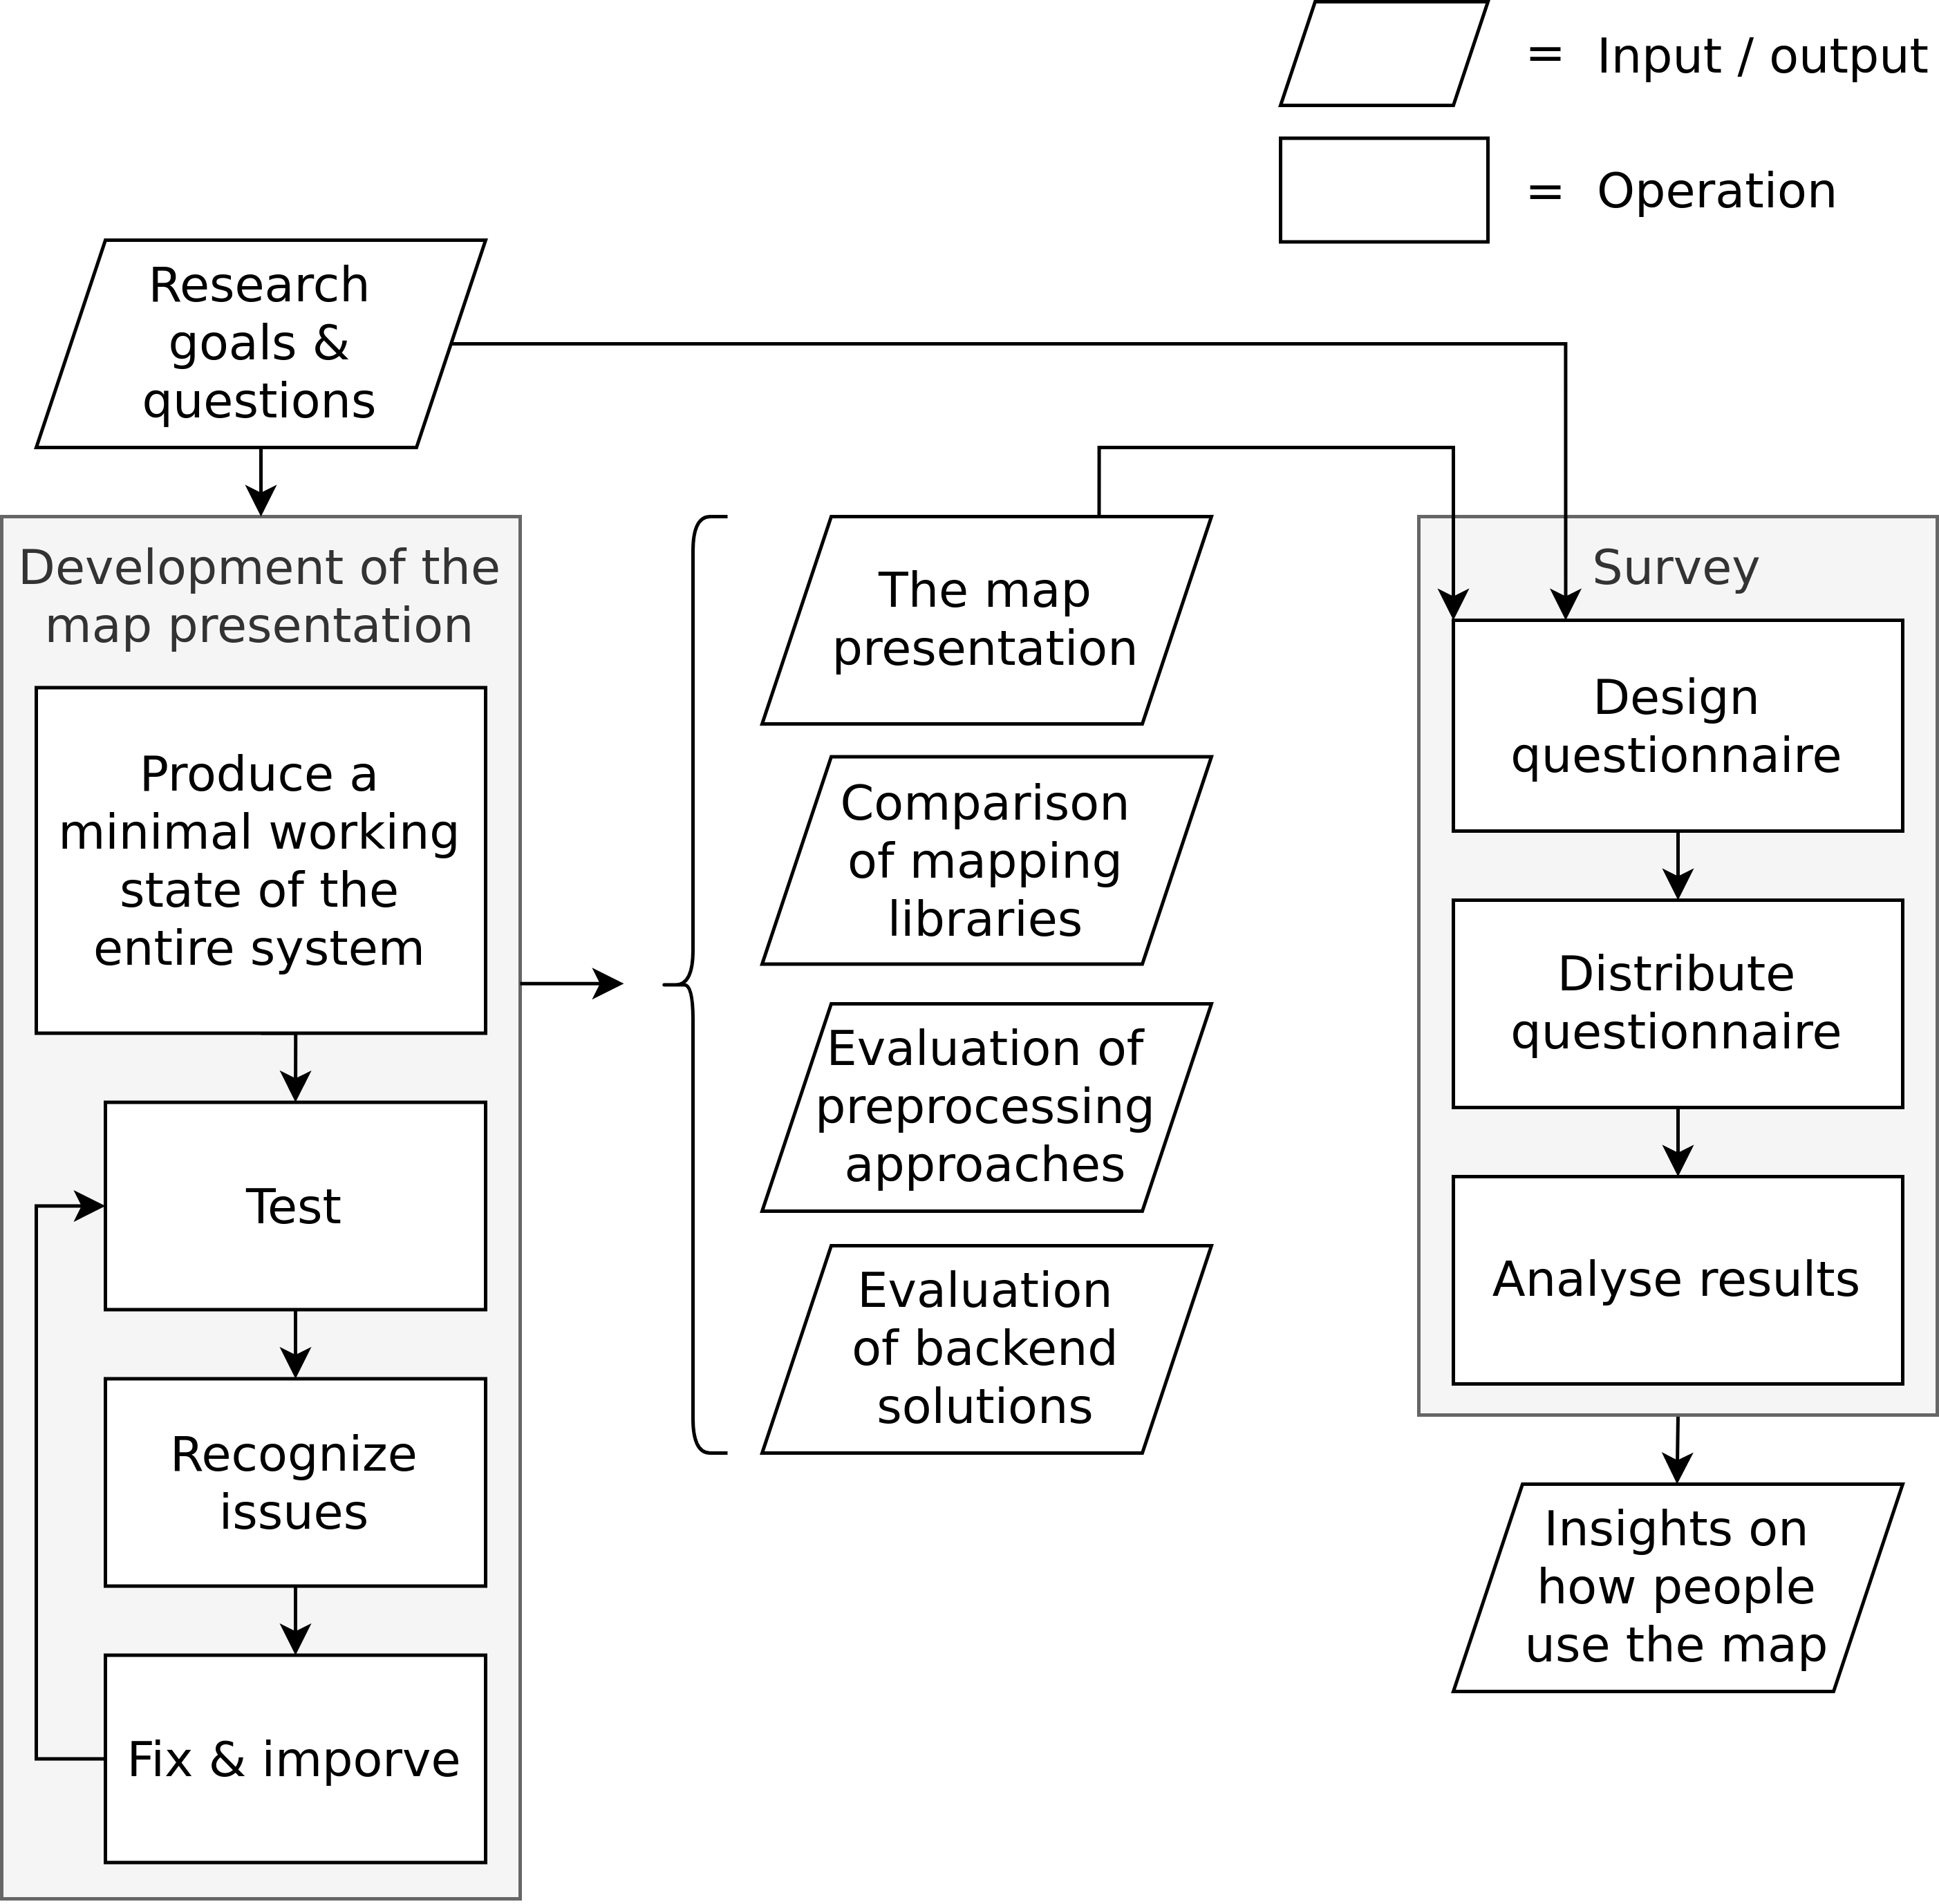
\includegraphics[width=0.8\textwidth]{visual/figures/diagrams/study_design.png}
	\caption{The design of the study}
	\label{fig:study design}
\end{figure}


\subsection{Data -- Helsinki region Travel Time Matrix}

The \acrlong{ttm} (\acrshort{ttm}) \parencite{fin2023}
is a dataset containing information of travel times and distances
in the Helsinki region in southern Finland.
This dataset is crucial to developing the map application,
as it is the sole source of the travel times shown on the map.

% Describe ttm in general: ykr, origin dest pairs etc (more surface level stuff common to all matrices)
A significant component of the \acrshort{ttm} is the \acrlong{ykr} (\acrshort{ykr})
statistical grid made by the Finnish Environmental Institute.
The grid has a spatial resolution of 250x250m, and it covers the entire Finland.
Most importantly, however, the part of the \acrshort{ykr} grid that overlaps with
the Helsinki region provides the spatial component for
the travel times stored in the \acrshort{ttm}.
The spatial extent of the dataset is shown in \ref{fig:ttm extent}.

\begin{figure}[H]
	\centering
	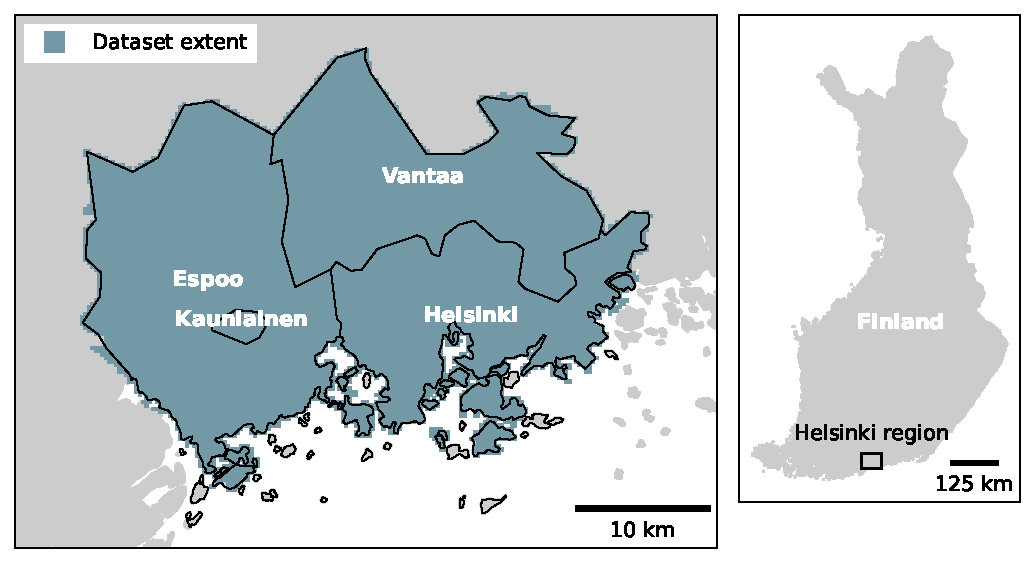
\includegraphics[width=0.8\textwidth]{visual/figures/ttm/ttm_extent.pdf}
	\caption{The location and extent of the TTM}
	\label{fig:ttm extent}
\end{figure}

The basic idea of the \acrshort{ttm} is that it stores the travel times and distances
from every \acrshort{ykr} grid cell to every grid cell within the Helsinki region.
The Helsinki region fits 13231 \acrshort{ykr} grid cells,
which means that the complete \acrshort{ttm} contains travel times and distances for
over 175 million routes.

All the routes are calculated for multiple different travel modes.
The primary travel modes are walking, cycling, public transportation and private car,
and, when applicable, each mode has variations based on
time of day and / or walking or cycling speed.
Time of day is especially relevant to motorized transport
in the form of the rush hour, for example,
while walking speed affects any travel mode
where a significant portion of the trip is covered on foot.
See table \ref{tab:ttm description} 

% TODO talk briefly about methodology, open source

% Describe the particular matrix (2023), methodology etc
There are matrices from many years.
This visualization is based on the 2023 version of the \acrshort{ttm}
\parencite{fin2023}.
The version of the \acrshort{ttm} used in this visualization is at the time of writing the newest one

\ref{tab:ttm description}

\begin{table}[H]
	\caption{Descriptive values of the \acrshort{ttm}}
	\label{tab:ttm description}
	\centering
	\begin{tabular}{ | L{0.4\textwidth} | L{0.5\textwidth} | }
		\hline
		Spatial resolution
		& 250 x 250 m
		\\
		\hline
		Number of grid cells
		& 13231
		\\
		\hline
		Number of origin-destination pairs
		& 175 059 361
		\\
		\hline
		Travel modes
		& \tabitem walking \\
		& \tabitem cycling \\
		& \tabitem public transportation \\
		& \tabitem private car \\
		\hline
		Travel mode variations (if applicable)
		& \tabitem Time of day (rush hour, midday, night) \\
		& \tabitem Walking speed (average, slow) \\
		& \tabitem Cycling speed (average, fast, slow) \\
		\hline
	\end{tabular}
\end{table}


\ref{tab:ttm table structure}

\begin{table}[H]
	\caption{The table structure of \acrshort{ttm} data}
	\label{tab:ttm table structure}
	\centering
	\begin{tabular}{ | L{0.15\textwidth} | L{0.75\textwidth} | }
		\hline
		\textbf{Column name}
		& \textbf{Description}
		\\
		\hline
		\hline
		from\_id
		& ID number of the origin grid cell
		\\
		\hline
		to\_id
		& ID number of the destination grid cell
		\\
		\hline
		walk\_avg
		& Travel time in minutes from origin to destination by walking at an average speed
		\\
		\hline
		walk\_slo
		& Travel time in minutes from origin to destination by walking slowly
		\\
		\hline
		bike\_avg
		& Travel time in minutes from origin to destination by cycling at an average speed; incl. extra time (1 min) to unlock and lock bicycle
		\\
		\hline
		bike\_fst
		& Travel time in minutes from origin to destination by cycling fast; incl. extra time (1 min) to unlock and lock bicycle
		\\
		\hline
		bike\_slo
		& Travel time in minutes from origin to destination by cycling slowly; incl. extra time (1 min) to unlock and lock bicycle
		\\
		\hline
		pt\_r\_avg
		& Travel time in minutes from origin to destination by public transportation in rush hour traffic, walking at an average speed
		\\
		\hline
		pt\_r\_slo
		& Travel time in minutes from origin to destination by public transportation in rush hour traffic, walking at a slower speed
		\\
		\hline
		pt\_m\_avg
		& Travel time in minutes from origin to destination by public transportation in midday traffic, walking at an average speed
		\\
		\hline
		pt\_m\_slo
		& Travel time in minutes from origin to destination by public transportation in midday traffic, walking at a slower speed
		\\
		\hline
		pt\_n\_avg
		& Travel time in minutes from origin to destination by public transportation in nighttime traffic, walking at an average speed
		\\
		\hline
		pt\_n\_slo
		& Travel time in minutes from origin to destination by public transportation in nighttime traffic, walking at a lower speed
		\\
		\hline
		car\_r
		& Travel time in minutes from origin to destination by private car in rush hour traffic
		\\
		\hline
		car\_m
		& Travel time in minutes from origin to destination by private car in midday traffic
		\\
		\hline
		car\_n
		& Travel time in minutes from origin to destination by private car in nighttime traffic
		\\
		\hline
		walk\_d
		& Distance from origin to destination, in metres, on foot
		\\
		\hline
	\end{tabular}
\end{table}




\subsection{Implementation of the map presentation}

\subsubsection{Software requirements}
% What interaction should there be in the map
% What requirements do the two above chapters place on the map

% Why this must be considered
% As mentioned earlier, cartographic visualization is often about tradeoffs.
% The interactive map crafted here is no exception.  % TODO
Before describing the development process,
I specify the requirements the system must meet.
I base these requirements on the goals of the study,
especially considering the interactive map presentation.
The requirements of the system are an essential aspect to consider,
since they  % TODO
For example, the sheer scale and detail of the dataset being visualized
means that instantaneous interaction with the map is not realistic
if no detail of the mapped data is to be sacrificed.
These kinds of tradeoffs are important to recognize,
because only through them is it possible to specify what
requirements should, or even could, be placed on the map application.

% By clearly stating the requirements I hope to
% more clearly justify the decisions
% I make in the technical portion of the study,
% TODO copypasta
Software requirements are often divided into
functional and nonfunctional requirements.
Functional requirements define the user-facing features of the system
while nonfunctional requirements describe the properties of a system
\parencite{chu2009}.
Nonfunctional requirements can be further divided into
quality attributes and constraints.
Quality attributes describe \textit{how} the software should be,
while constraints mean technical limitations \parencite{chu2009}.

% Roughly what kind of a map? Why?
% Based on the background study,  % TODO
The starting point for specifying the requirements of the system
Was the decision to prioritize real-time interaction over minute detail in the map.
The goal of the map is to act as a dynamic overview to the entire \acrshort{ttm},
and user interaction, whether it is changing the location or travel mode to view,
should result in instant visual feedback on the map.

This goal immediately placed a number of requirements on the system.
From the perspective of the user,
there must be functionalities for interacting with the map to
select different locations and travel modes.
A significant quality attribute to consider is that the system should
support real-time interactivity.
To achieve this, the latency between user input and
its visible results must be minimized.
In this particular system latency is introduced by transferring data over the

This decision is what ultimately shapes the requirements for the mapped data,
and thus dictates what kind of processing should be done on the data.

After the implementation of the minimal working system, these requirements


\ref{tab:functional requirements}

\begin{table}[H]
	\caption{The functional requirements of the map application}
	\label{tab:functional requirements}
	\centering
	\begin{tabular}{ | L{0.3\textwidth} | L{0.6\textwidth} | }
		\hline
		Requirement
		& Description
		\\
		\hline
		\hline
		Location selection by clicking
		& The user can click on a location and produce an accessibility map of that location.
		\\
		\hline
		Location selection by hovering
		& The user can hover their mouse over the map,
		and the map shows the accessibility of the location that is under the cursor,
		updating constantly as the cursor moves.
		\\
		\hline
		Toggling between modes of location selection
		& The user can toggle their mode of interaction by clicking:
		Clicking while hovering locks the map, clicking while the map is locked resumes hovering.
		\\
		\hline
		Interactive selection of travel mode
		& The user can choose the travel mode for which the travel times shown on the map are calculated.
		\\
		\hline
	\end{tabular}
\end{table}


\ref{tab:nonfunctional requirements}

\begin{table}[H]
	\caption{
		The nonfunctional requirements of the map application specify
		its desired qualities (\ref{tab:quality attributes}) and
		the constraints it must adhere to (\ref{tab:constraints}).
	}
	\label{tab:nonfunctional requirements}
	\begin{subtable}[h]{\textwidth}
		\caption{}
		\label{tab:quality attributes}
		\centering
		\begin{tabular}{ | L{0.2\textwidth} | L{0.7\textwidth} | }
			\hline
			\textbf{Category}
			& \textbf{Requirements}
			\\
			\hline
			\hline
			Performance
			& \tabitem Data serving speed allows for real-time interaction. \\
			& \tabitem Map rendering speed allows for real-time interaction. \\
			\hline
			Maintainability
			& \tabitem All components are as independent as possible. \\
			& \tabitem The codebase is versioned and documented. \\
			& \tabitem Deploying the application is reproducible. \\
			\hline
			Usability
			& \tabitem Visual feedback from user interaction is instantaneous. \\
			\hline
			Scalability
			& \tabitem The application is scalable to meet different usage loads. \\
			& \tabitem Different application components can be scaled independently. \\
			\hline
		\end{tabular}
	\end{subtable}
	\newline
	\newline  % https://tex.stackexchange.com/questions/38893/cant-generate-vertical-space-between-tables
	\newline
	\begin{subtable}[h]{\textwidth}
		\caption{}
		\label{tab:constraints}
		\centering
		\begin{tabular}{ | L{0.2\textwidth} | L{0.7\textwidth} | }
			\hline
			\textbf{Type of constraint}
			& \textbf{Description}
			\\
			\hline
			\hline
			Client-side platform
			& The frontend of the map application runs in a web browser.
			\\
			\hline
			Deployment environment
			& The front and backend are deployed in containers
			utilizing the OpenShift container platform.
			\\
			\hline
		\end{tabular}
	\end{subtable}
\end{table}


See figure \ref{fig:architechture} for the architecture.

\begin{figure}[H]
	\centering
	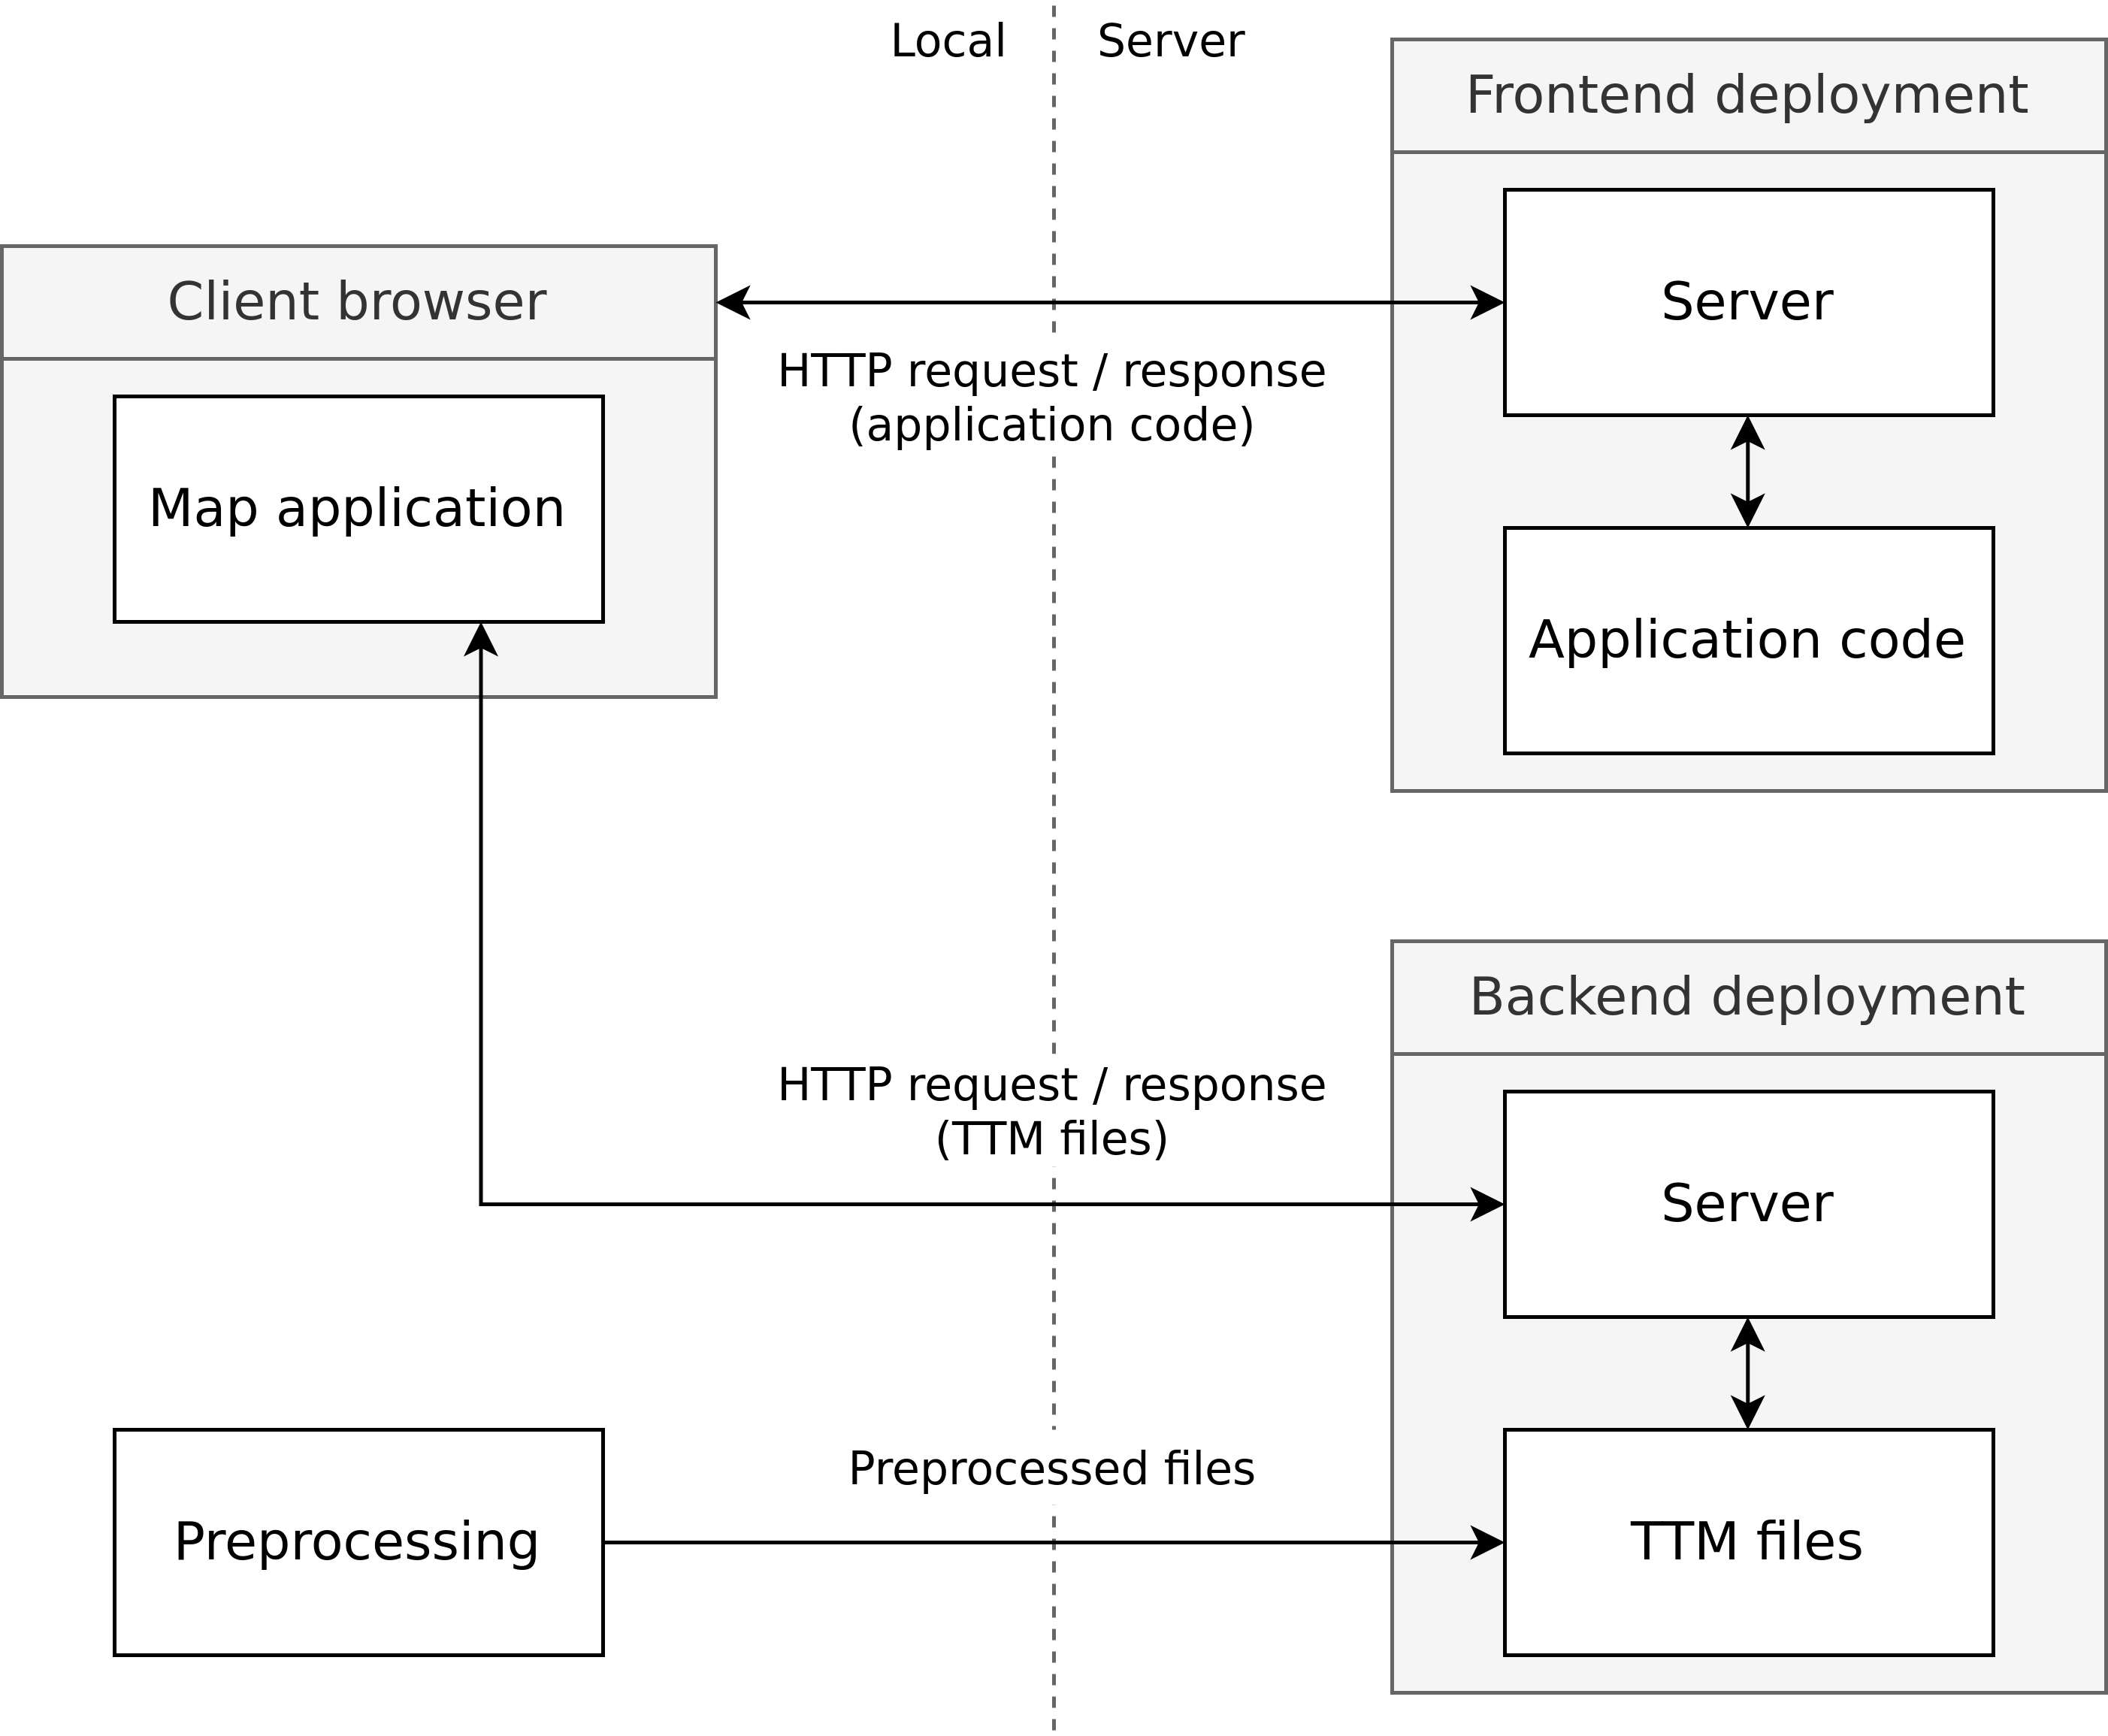
\includegraphics[width=0.8\textwidth]{visual/figures/diagrams/architechture.png}
	\caption{Architecture}
	\label{fig:architechture}
\end{figure}

\subsubsection{Data preprocessing}
Considering the requirements, the \acrshort{ttm}
To make the \acrshort{ttm} mappable, it must be at some point of the
To enable real-time interactivity with the map the travel time

% The need for preprocessing
% - what would raw data be like?
% - why as much as possible should be precalculated
% && the requirements preprocessing must satisfy

% Different approaches

% Why isochrones?

% Describe how it was done

See figure \ref{fig:preprocessing} for preprocessing.

\begin{figure}[H]
	\centering
	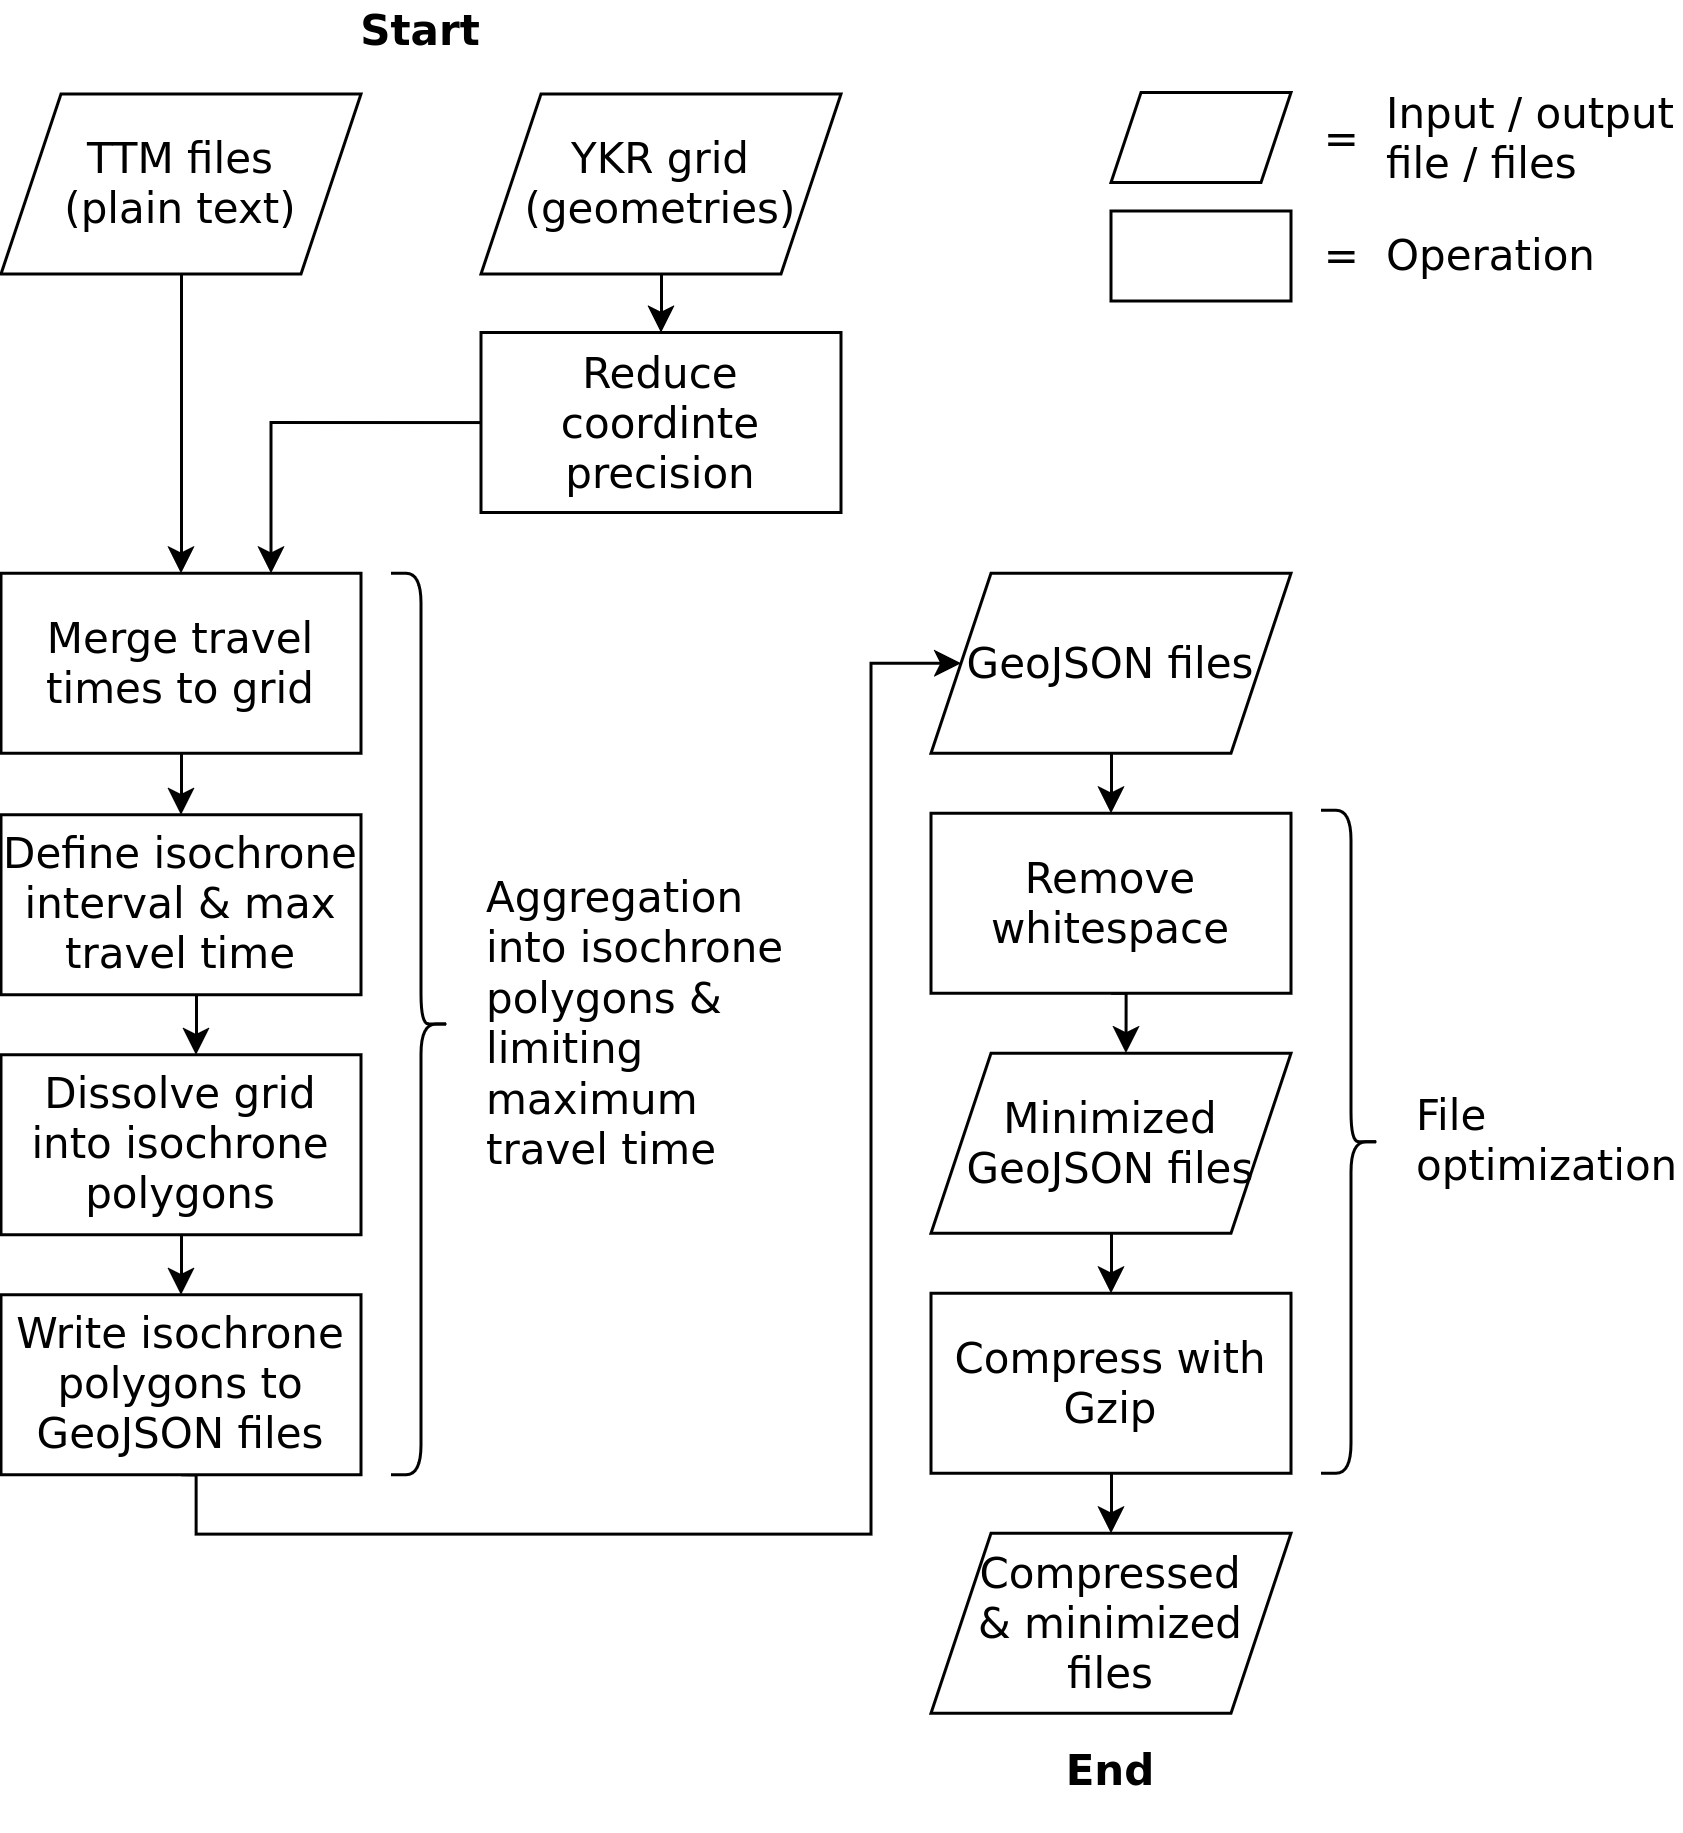
\includegraphics[width=0.8\textwidth]{visual/figures/diagrams/preprocessing.png}
	\caption{Preprocessing}
	\label{fig:preprocessing}
\end{figure}


\subsubsection{Constructing the map application}

The need for visualization (frontend) and the requirements visualization must satisfy

Different approaches

Why react? Why not just make a map?
The map is a map, but it is also a user interface that controls state outside the map.
Integration with react means more robust code, better developer experience and maintainability.
Do not reinvent the wheel.

% TODO Describe why these libraries were selected
Basis for the map library comparison

Baseline: FOSS, Actively maintained, usable with UI framework (react)

Initial contenders: Leaflet, Openlayers, Mapbox, Maplibre, Deckgl

Instantly discarded: Openlayers (non-existent integration to react) Mapbox (non-foss)

% TODO copypasta
Translucent Overlay (OV) is the best technique over-
all, which makes it a good choice when only one comparison
technique should be provided to user \parencite{lob2015}.

% Describe how it was done



% I see the methods necessary to implement the visualisation belonging to two themes:
% Methods for figuring out how the map should be
% and methods for actually making the map be that way.

% For figuring out what the map should be like,
% I have (hopefully) at this point already formed some ideas from the background section.
% To complement those, and to keep the qualitative aspect of cartography relevant,
% interview(s) will be used alongside the development process.

% When developing the visualisation, the priority should be on the map application.
% However, the development must progress on all components as an iterative process,
% where producing a minimal working state should be the first goal.
% Something that, to some extent, works, makes discussion about the map possible,
% which in turn should keep development progressing towards the right direction.

% It should also be noted that the number of techical options for implementing the map is large.
% Questions such as which mapping library or UI framework to use,
% or how to preprocess the matrix data should be covered here too.
% Depending on the need and extent of comparisons between different technologies,
% some synthesis could be formed about that too.

\subsubsection{Technical architecture}

% The need for serving (backend)
% - why data must be decoupled
% && the requirements serving must satisfy

% Different approaches

% Why nginx + static files?

% Describe how it was done

\subsection{Survey}
General reasoning about the survey

\subsubsection{Questionnaire design and structure}
The content of the questionnaire: prompts and questions

\subsubsection{Survey process}
The content of the questionnaire: prompts and questions

\subsubsection{Participants}
Descrtiption of the collected data
